\documentclass[12pt]{report}
\usepackage[utf8]{inputenc}
\usepackage[russian]{babel}
%\usepackage[14pt]{extsizes}
\usepackage{listings}
\usepackage{graphicx}
\usepackage{amsmath,amsfonts,amssymb,amsthm,mathtools} 
\usepackage{pgfplots}
\usepackage{filecontents}
\usepackage{indentfirst}
\usepackage{eucal}
\usepackage{amsmath}
\usepackage{enumitem}
\frenchspacing

\usepackage{indentfirst} % Красная строка


%\usetikzlibrary{datavisualization}
%\usetikzlibrary{datavisualization.formats.functions}

\usepackage{amsmath}




% Для листинга кода:
\lstset{ %
language=haskell,                 % выбор языка для подсветки (здесь это С)
basicstyle=\small\sffamily, % размер и начертание шрифта для подсветки кода
numbers=left,               % где поставить нумерацию строк (слева\справа)
numberstyle=\tiny,           % размер шрифта для номеров строк
stepnumber=1,                   % размер шага между двумя номерами строк
numbersep=5pt,                % как далеко отстоят номера строк от подсвечиваемого кода
showspaces=false,            % показывать или нет пробелы специальными отступами
showstringspaces=false,      % показывать или нет пробелы в строках
showtabs=false,             % показывать или нет табуляцию в строках
frame=single,              % рисовать рамку вокруг кода
tabsize=2,                 % размер табуляции по умолчанию равен 2 пробелам
captionpos=t,              % позиция заголовка вверху [t] или внизу [b] 
breaklines=true,           % автоматически переносить строки (да\нет)
breakatwhitespace=false, % переносить строки только если есть пробел
escapeinside={\#*}{*)}   % если нужно добавить комментарии в коде
}

\usepackage[left=2cm,right=2cm, top=2cm,bottom=2cm,bindingoffset=0cm]{geometry}
% Для измененных титулов глав:
\usepackage{titlesec, blindtext, color} % подключаем нужные пакеты
\definecolor{gray75}{gray}{0.75} % определяем цвет
\newcommand{\hsp}{\hspace{20pt}} % длина линии в 20pt
% titleformat определяет стиль
\titleformat{\chapter}[hang]{\Huge\bfseries}{\thechapter\hsp\textcolor{gray75}{|}\hsp}{0pt}{\Huge\bfseries}


% plot
\usepackage{pgfplots}
\usepackage{filecontents}
\usetikzlibrary{datavisualization}
\usetikzlibrary{datavisualization.formats.functions}

\begin{document}
%\def\chaptername{} % убирает "Глава"
\thispagestyle{empty}
\begin{titlepage}
	\noindent \begin{minipage}{0.15\textwidth}
	
\includegraphics[width=\linewidth]{b_logo}
	\end{minipage}
	\noindent\begin{minipage}{0.9\textwidth}\centering
		\textbf{Министерство науки и высшего образования Российской Федерации}\\
		\textbf{Федеральное государственное бюджетное образовательное учреждение высшего образования}\\
		\textbf{~~~«Московский государственный технический университет имени Н.Э.~Баумана}\\
		\textbf{(национальный исследовательский университет)»}\\
		\textbf{(МГТУ им. Н.Э.~Баумана)}
	\end{minipage}
	
	\noindent\rule{18cm}{3pt}
	\newline\newline
	\noindent ФАКУЛЬТЕТ $\underline{\text{«Информатика и системы управления»}}$ \newline\newline
	\noindent КАФЕДРА $\underline{\text{«Программное обеспечение ЭВМ и информационные технологии»}}$\newline\newline\newline\newline\newline
	
	
	\begin{center}
		\noindent\begin{minipage}{1.3\textwidth}\centering
			\Large\textbf{  Отчёт по лабораторной работе №4}\newline
			\textbf{по дисциплине "Анализ алгоритмов"}\newline\newline
		\end{minipage}
	\end{center}
	
	\noindent\textbf{Тема} $\underline{\text{Исследование многопоточности}}$\newline\newline
	\noindent\textbf{Студент} $\underline{\text{Варламова Е. А.}}$\newline\newline
	\noindent\textbf{Группа} $\underline{\text{ИУ7-51Б}}$\newline\newline
	\noindent\textbf{Оценка (баллы)} $\underline{\text{~~~~~~~~~~~~~~~~~~~~~~~~~~~}}$\newline\newline
	\noindent\textbf{Преподаватели} $\underline{\text{Волкова Л.Л.}}$\newline\newline\newline
	
	\begin{center}
		\vfill
		Москва~---~\the\year
		~г.
	\end{center}
\end{titlepage}

\setcounter{page}{2}
\tableofcontents

\newpage
\chapter*{Введение}
\addcontentsline{toc}{chapter}{Введение}

Поток или поток выполнения - базовая упорядоченная последовательность инструкций, которые могут быть переданы или обработаны одним ядром процессора. Вычисления разбиваются на части, за каждую из которых отвечает отдельный поток. Если в системе больше одного процессора, то использование многопоточности фактически позволяет выполнять несколько действий одновременно.

Многие алгоритмы (операции над матрицами, алгоритмы компьютерной графики) допускают многопоточную реализацию. Поэтому \textbf{целью} данной работы является сравнить производительность обычной и многопоточной реализаций алгоритма трассировки лучей.
Для достижения поставленной цели необходимо решить следующие задачи.
\begin{enumerate}
    \item Выбрать метод распараллеливания алгоритма трассировки лучей.
	\item Реализовать однопоточный алгоритм трассировки лучей.
	\item Реализовать многопоточный алгоритм трассировки лучей.
	\item Протестировать реализованные алгоритмы.
	\item Провести сравнительный анализ алгоритмов по времени выполнения в зависимости от количества потоков.
\end{enumerate}

\chapter{Аналитическая часть}

\section{Трассировка лучей}

Трассировка лучей – метод синтеза компьютерных изображений. Основная идея, лежащая в основе этого метода заключается в том, что наблюдатель видит любой объект посредством испускаемого неким источником света, который  падает на этот объект и затем доходит до наблюдателя. Если проследить за лучами, испущенными источником света, то лишь немногие из них дойдут до наблюдателя. Поэтому предлагается отслеживать лучи в обратном направлении, то есть от наблюдателя к объекту[1]. В алгоритме предполагается, что наблюдатель находится на оси z, а картинная плоскость (растр) перпендикулярна ей. Для каждого пиксела в итоговом изображении математический луч испускается из положения наблюдателя через растр в направлении к объектам сцены. Тогда для каждого луча необходимо найти все пересечения с объектами сцены и выбрать ближайшее к наблюдателю. Это пересечение и будет являться видимой наблюдателю частью объекта. Для учёта освещения, отражения, прозрачности, теней и блеска объектов используется тот же алгоритм трассировки, но лучи испускаются не из положения наблюдателя, а из точки на поверхности объектов. 

Алгоритм трассировки лучей требует большого количества вычислений, поскольку он предполагает поиск пересечений всех объектов сцены со всеми лучами, количество которых равно размеру растра. Поэтому время синтеза изображения оказывается очень большим. Однако из описания алгоритма видно, что вычисление цвета каждого пиксела может быть выполнено параллельно. Такая оптимизация позволит значительно ускорить синтез изображения.

\section{Вывод}
	В данном разделе был расссмотрен алгоритм трассировки лучей и выбран метод распараллеливания вычислений.
\clearpage

\chapter{Конструкторская часть}

На рисунках \ref{fig:one} и \ref{fig:multi} приведены схемы однопоточного и многопоточного синтеза изображения, в основе которого лежит алгоритм трассировки лучей. На рисунке  \ref{fig:base} приведена схема алгоритма трассировки лучей.

\section{Схемы алгоритмов}

\begin{figure}[h!p]
	\centering
	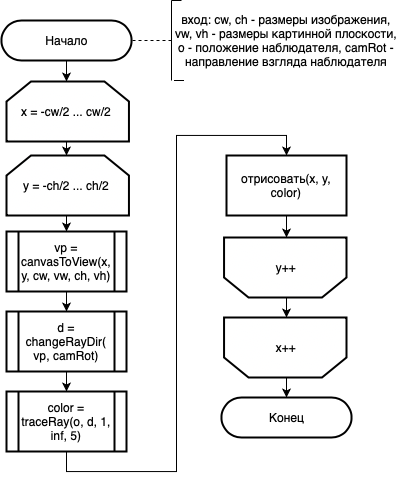
\includegraphics[scale = 0.7]{one.drawio.png}
	\caption{Схема однопоточного синтеза изображения}
	\label{fig:one}
\end{figure}
\begin{figure}[h!p]
	\centering
	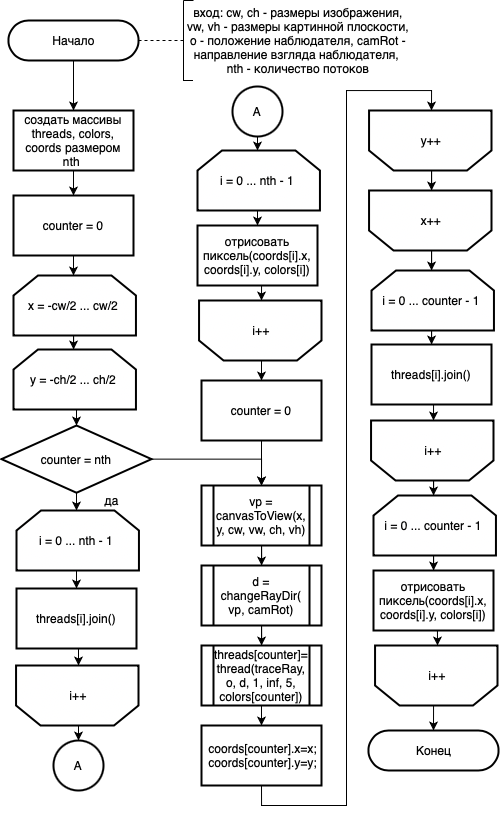
\includegraphics[scale = 0.75]{multi.drawio.png}
	\caption{Схема однопоточного синтеза изображения}
	\label{fig:multi}
\end{figure}

\begin{figure}[h!p]
	\centering
	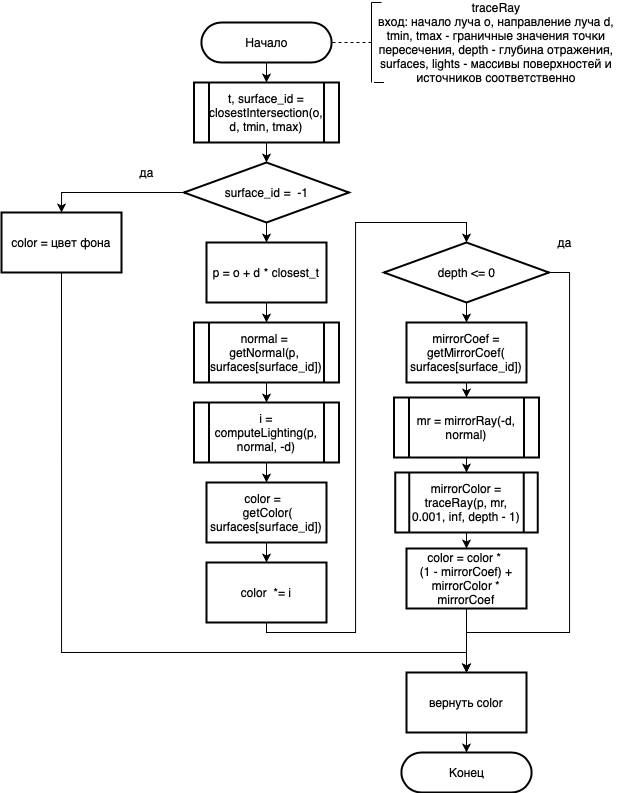
\includegraphics[scale = 0.7]{base.drawio.png}
	\caption{Схема алгоритма трассировки лучей}
	\label{fig:base}
\end{figure}

\section{Вывод}
На основе анализа алгоритма трассировки лучей были построены схемы однопоточного и многопоточного синтеза изображения. 

\chapter{Технологическая часть}

В данном разделе приведены средства реализации и листинги кода.

\section{Средства реализации}
Для реализации был выбран язык программирования C++. Данный выбор обусловлен наличием инструментов для создания и эффективной работы с потоками. В качестве среды разработки была выбрана среда CLion.

\section{Реализация алгоритмов}

В листингах \ref{one_code}, \ref{multi_code} и \ref{base_code} приведены реализации однопоточного, многопоточного синтеза изображения и алгоритма трассировки лучей соответственно.

\begin{lstlisting}[label=one_code,caption=Однопоточный синтез изображения,language=C]
void View::drawScene(int cw, int ch, double vw, double vh, Point &o, Matrix<double> &camera_rotation)
{
    int planeZ = 1;
    scene->clear();
    for (int x = -cw / 2; x <= cw / 2; x++)
    {
        for (int y = -ch / 2; y <= ch / 2; y++)
        {
            Point viewportPoint(canvas_to_viewport(x, cw, vw),
                                canvas_to_viewport(y, ch, vh),
                                planeZ);
            Point d = changeRayDirection(viewportPoint, camera_rotation);
            QColor color;
            rt.traceRay(o, d, 1, INT_MAX, 1, color);
            scene->addRect(x, -y, 1, 1, QPen(color));
        }
    }
}

\end{lstlisting}
\newpage
\begin{lstlisting}[label=multi_code,caption=Многопоточный синтез изображения,language=C]
void View::drawSceneMulti(int cw, int ch, double vw, double vh, Point &o, Matrix<double> &camera_rotation, int nth)
{
    int planeZ = 1;
    scene->clear();
    std::vector <std::thread > threads(nth);
    std::vector<QColor> colors(nth);
    std::vector<pair<int, int>> coords(nth);
    int counter = 0;
    for (int x = -cw / 2; x <= cw / 2; x++)
    {
        for (int y = -ch / 2; y <= ch / 2; y++)
        {
            if (counter == nth)
            {
                for (int i = 0; i < nth; ++i) {
                    threads[i].join();
                }
                for (int i = 0; i < nth; ++i)
                    scene->addRect(coords[i].first, coords[i].second, 1, 1, QPen(colors[i]));
                counter = 0;
            }
            Point viewportPoint(canvas_to_viewport(x, cw, vw),
                                canvas_to_viewport(y, ch, vh),
                                planeZ);
            Point d = changeRayDirection(viewportPoint, camera_rotation);

            threads[counter] = std::thread(&RayTracer::traceRay, rt, o, d, 1, INT_MAX, 1, std::ref(colors[counter]));
            coords[counter] = std::pair<int, int>(x, -y);
            counter++;
        }
    }
    for (int i = 0; i < counter; ++i) {
        threads[i].join();
    }
    for (int i = 0; i < counter; ++i)
        scene->addRect(coords[i].first, coords[i].second, 1, 1, QPen(colors[i]));
}
\end{lstlisting}
\newpage
\begin{lstlisting}[label=base_code,caption=Алгоритм трассировки лучей, language=C]
QColor RayTracer::traceRay(Point o, Point d, double tmin, double tmax, int depth, QColor &tmp)
{
    int closest_surface;
    double closest_t;
    closestIntersection(o, d,  tmin, tmax, closest_surface, closest_t);
    if (closest_surface == -1) {
        tmp = QColor(0, 0, 0);
        return QColor(0, 0, 0);
    }
    Point p = o + d * closest_t;
    Point normal;
    surfaces[closest_surface]->getNormal(p, normal);

    double i = computeLighting(p, normal, -d, surfaces[closest_surface]->getShineCoef());
    QColor color = surfaces[closest_surface]->getColor();
    color = mulColor(color, i);

    double mirrorCoef = surfaces[closest_surface]->getMirrorCoef();
    if (!(depth <= 0 || mirrorCoef <= 0))
    {
        QColor mirrorColor = traceRay(p, mirrorRay(-d, normal), 0.001, INT_MAX, depth - 1, tmp);
        color = sumColor(mulColor(color, (1 - mirrorCoef)),
                         mulColor(mirrorColor, mirrorCoef));
    }

    tmp = color;
    return color;
}
\end{lstlisting}

\section{Тестирование}

При тестировании проверялась корректность изображений, полученных при работе программы с различными данными. Результаты представлены на \ref{fig:test1} и \ref{fig:test2}.

\begin{figure}[h!p]
	\centering
	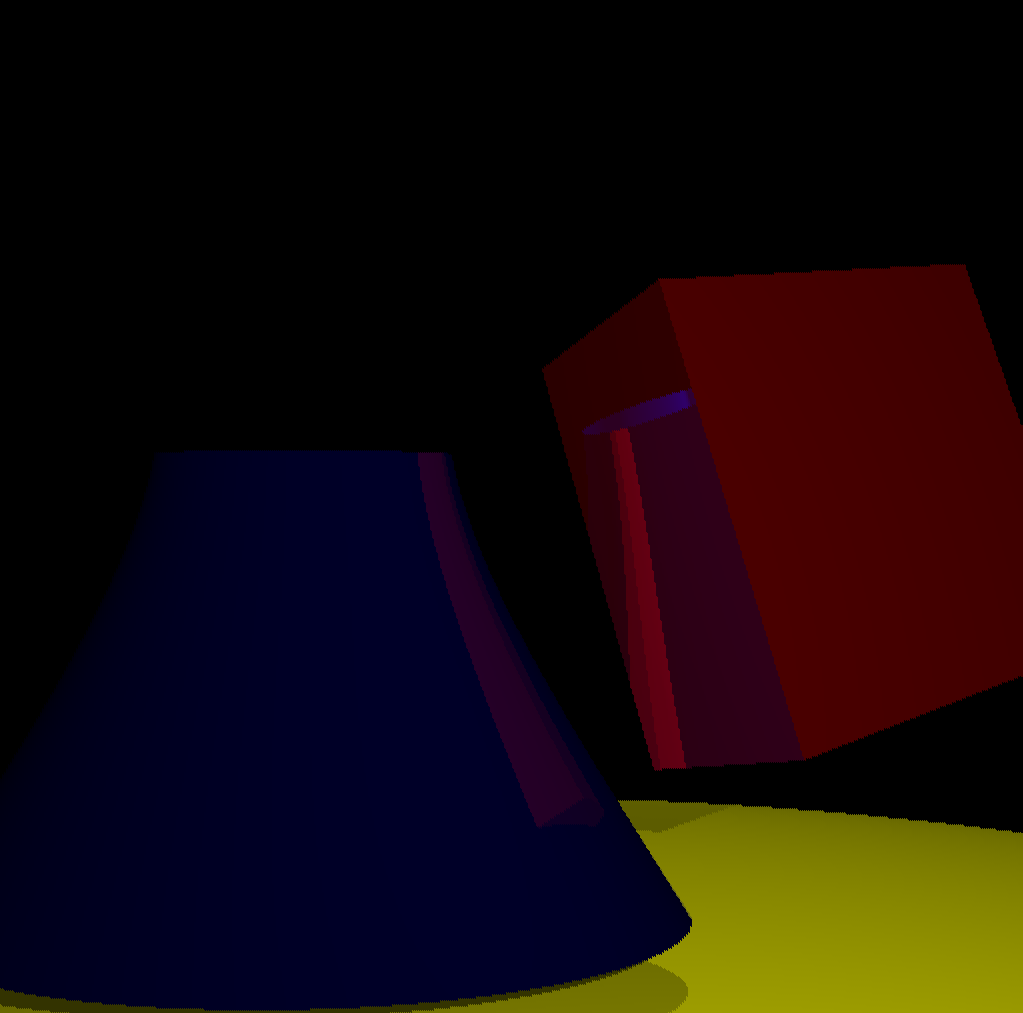
\includegraphics[scale = 0.6]{1.png}
	\caption{Взаимное отражение}
	\label{fig:test1}
\end{figure}
\begin{figure}[h!p]
	\centering
	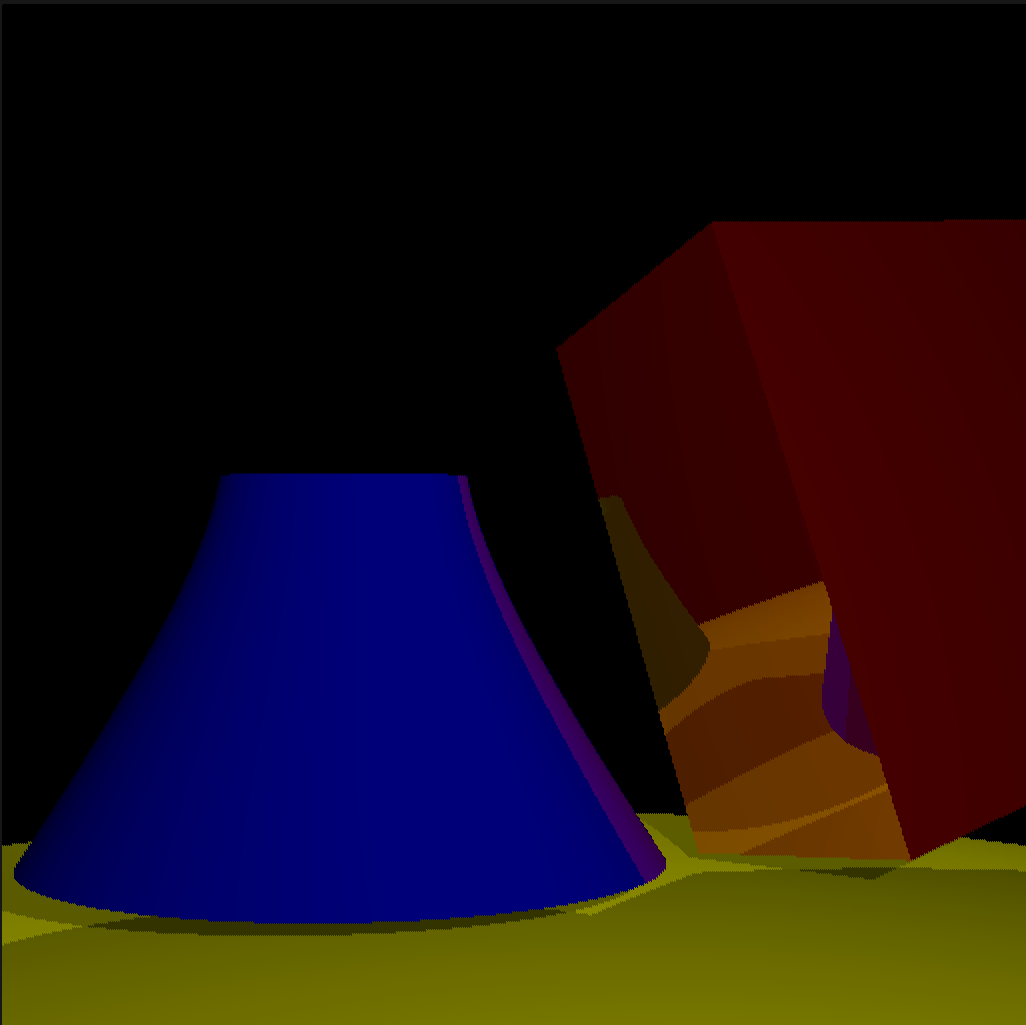
\includegraphics[scale = 0.6]{2.png}
	\caption{Зелёная поверхность, закрытая синей, видна в отражении куба}
	\label{fig:test2}
\end{figure}

Все тесты пройдены успешно.
\newpage
\section{Вывод}

В данном разделе были разработаны исходные коды алгоритмов: однопоточный и многопоточный алгоритмы трассировки лучей.

\chapter{Исследовательская часть}

\section{Технические характеристики}

Все нижепреведенные замеры времени проведены на процессоре: Intel Core i5, 1,4 GHz, 4ядерный, количество логических ядер - 8. Время работы алгоритмов было замерено с помощью time.h, функции clock, которая измеряет процессорное время [2].


\section{Время выполнения алгоритма}
В \ref{tableComp} приведено время выполнения алгоритма трассировки лучей при разных размерах изображения (от 100 * 100 до 500 * 500 пикселей) и разных количествах потоков (1, 2, 4, 8, 16, 32). На \ref{imageComp} показано то же самое в виде графика. Время на графике и в таблице указано в мс.

\begin{table} [h!]
    \label{tableComp}
	\caption{Таблица времени выполнения при разных размерах изображения и количествах потоков}
	\begin{center}
		\begin{tabular}{|c c c c c c|} 
			\hline
			Количество потоков &  100 * 100 & 200 * 200 & 300 * 300 & 400 * 400 & 500 * 500 \\  
            \hline
            1 & 1614.33 & 6333.63 & 14180.2 & 25329.2 & 39221.8\\
            \hline
            2 & 1045.01 & 4143.79 & 9655.59 & 17172.8 & 25637.5\\
            \hline
            4 & 545.895 & 2226.87 & 5155.55 & 9462.02 & 15123.8\\
            \hline
            8 & 374.916 & 1617.05 & 3743.16 & 6907.58 & 10955.2\\
            \hline
            16 & 409.756 & 1752.07 & 4057.03 & 7311.09 & 11746.3\\
            \hline
            32 & 421.671 & 1805.8 & 4087.55 & 7360.05 & 11631.2\\
			\hline
		\end{tabular}
	\end{center}
\end{table}
\newpage
\begin{figure}[h!p]
	\centering
	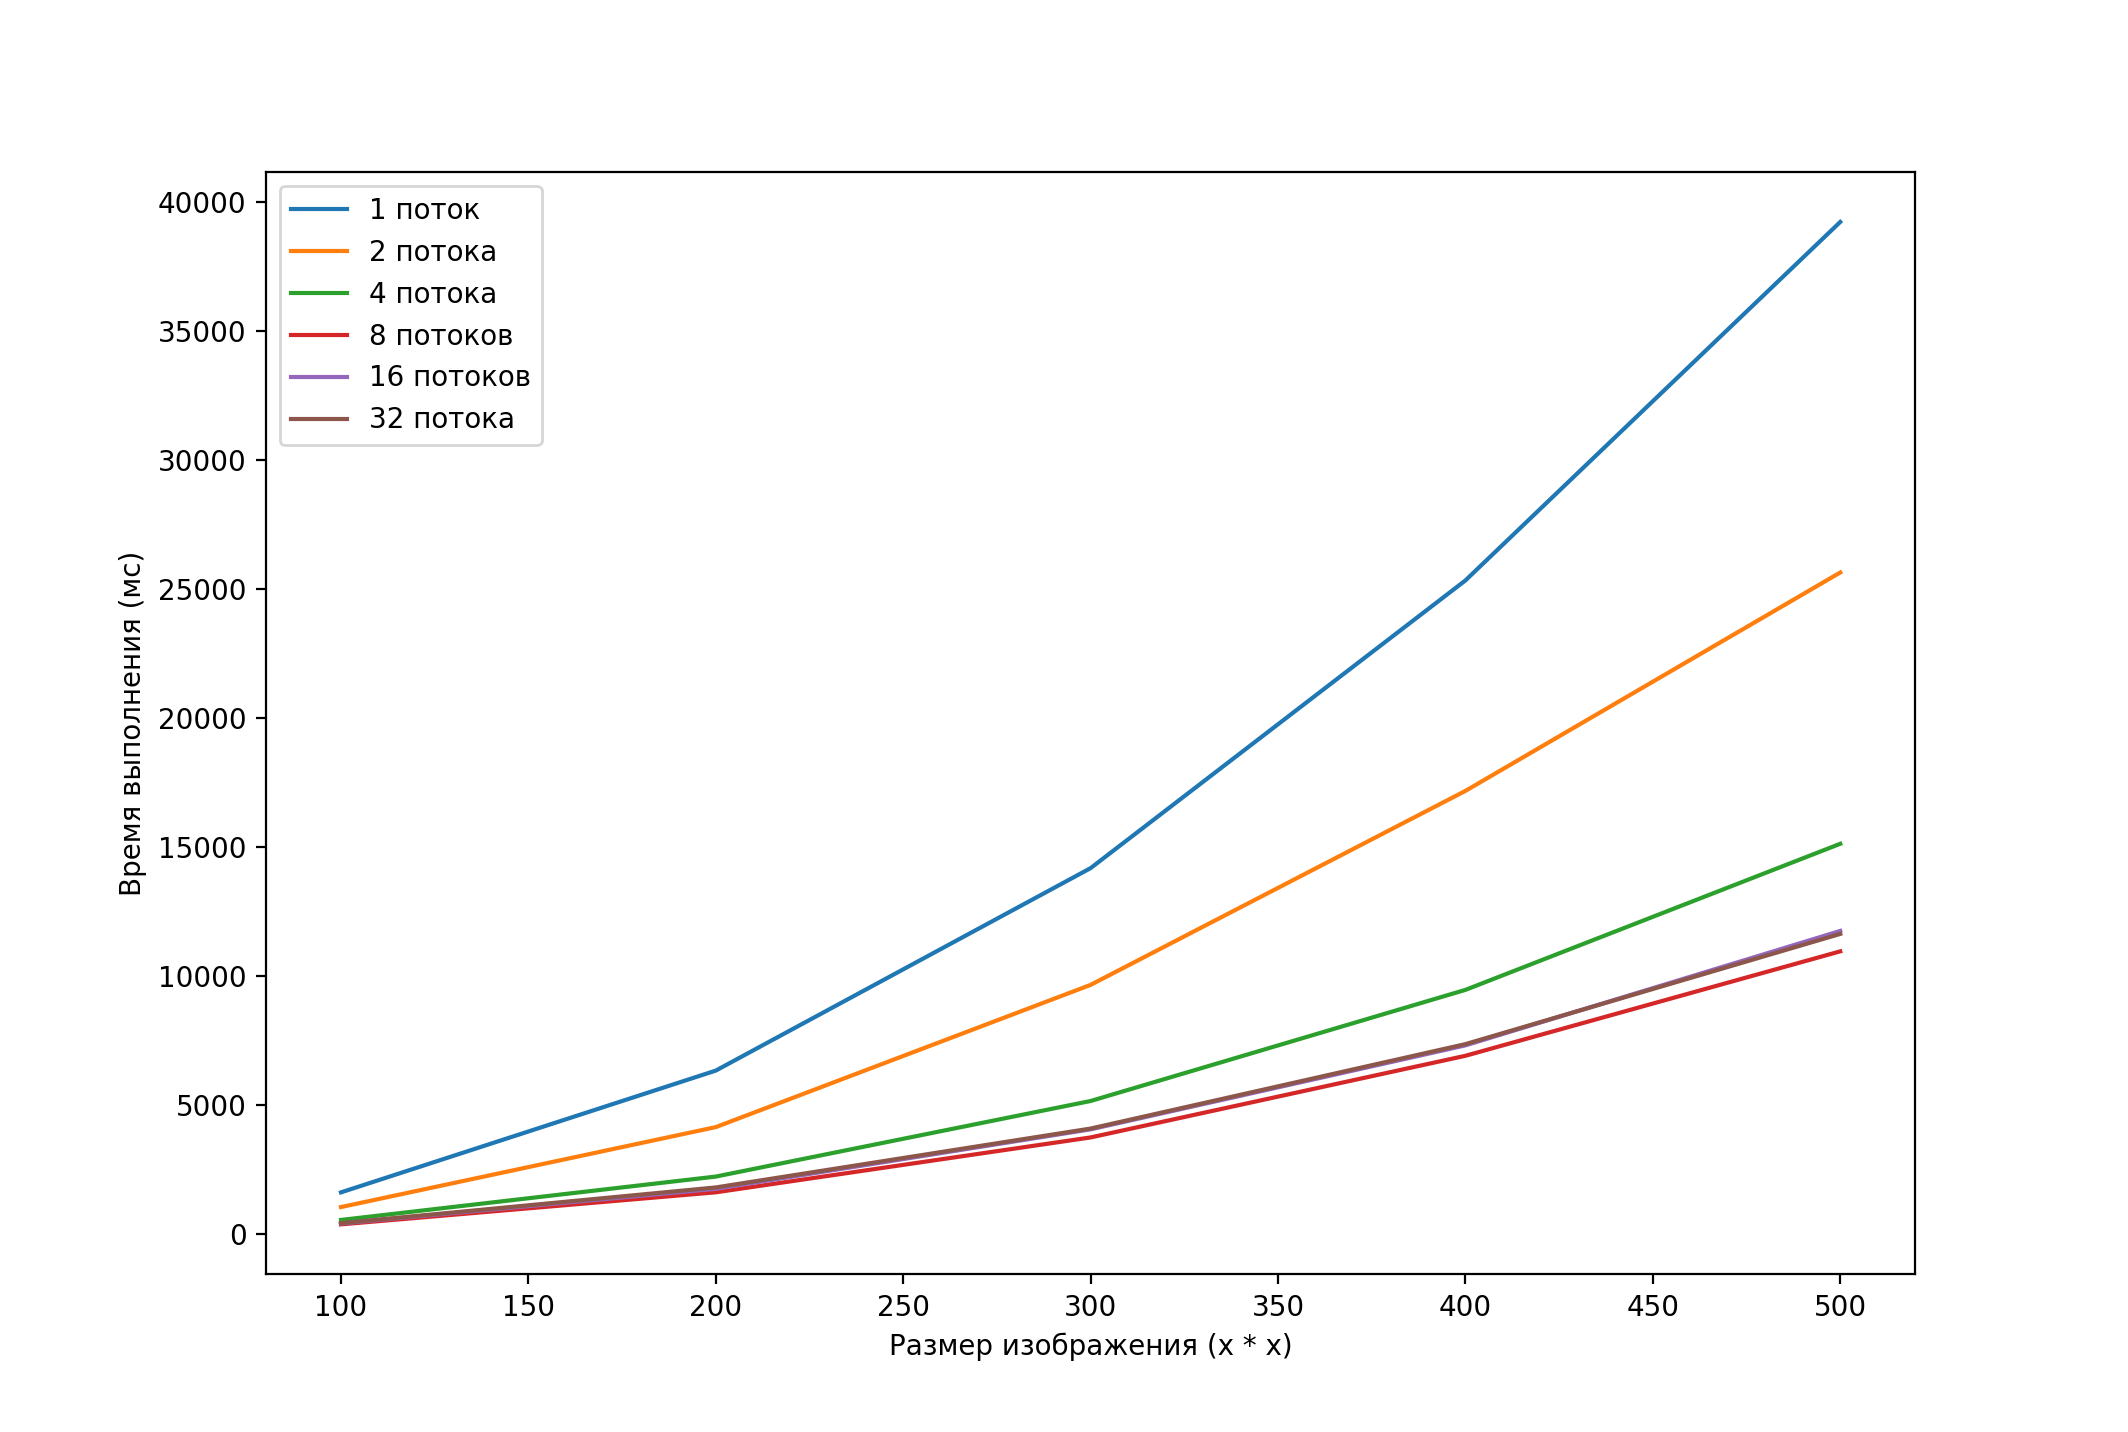
\includegraphics[scale = 0.7]{threadsComp.png}
	\caption{Зависимость времени выполнения от размера изображения при разных количествах потоков}
	\label{imageComp}
\end{figure}

\section{Вывод}

Наилучшее время параллельные алгоритмы показали при 8 потоках, что соответствует количеству логических ядер компьютера, на котором проводилось тестирование. На изображениях размером 500 на 500 пикселей, параллельный алгоритм с 8 потоками работает примерно в 3.6 раза быстрее однопоточной реализации. При количестве потоков, большем чем 8, время выполнения немного ухудшается по сравнению с реализацией с 8 потоками. 
\chapter*{Заключение}
\addcontentsline{toc}{chapter}{Заключение}

В рамках данной лабораторной работы были решены следующие задачи.

\begin{itemize}
    \item Выбран метод распараллеливания алгоритма трассировки лучей.
	\item Реализован однопоточный алгоритм трассировки лучей.
	\item Реализован многопоточный алгоритм трассировки лучей.
	\item Протестированы реализованные алгоритмы.
	\item Проведён сравнительный анализ алгоритмов по времени выполнения в зависимости от количества потоков.
\end{itemize}

В результате исследования было выяснено, что параллельные реализации алгоритма трассировки лучей работают быстрее однопоточной реализации. Наиболее эффективны данные алгоритмы при количестве потоков, совпадающем с количеством логических ядер компьютера. Так, например, на изображениях размером 500 на 500, удалось улучшить время выполнения алгоритма в 3.6 раз (в сравнении с однопоточной реализацией).

Поставленная цель была достигнута.

\chapter*{Литература}
\addcontentsline{toc}{chapter}{Литература}
\begin{enumerate}
    \item Роджерс Д., Адамс Дж. Математические основы машинной графики. М.: Мир, 2001. 604 с.
	\item Стандартная функция clock(), измеряющая процессорное время [Электронный ресурс]. Режим доступа: https://en.cppreference.com/w/cpp/chrono/c/clock. Дата обращения: 19.10.2021
	
\end{enumerate}

\end{document}